\documentclass{article}

%\usepackage{minted}
\usepackage{tikz}
\usetikzlibrary{automata, positioning, arrows}
\usepackage{graphicx}
\usepackage{geometry}
\geometry {
    top=25mm,
    bmargin=25mm,
}

\begin{document}

\begin{titlepage}
    \centering
    \hrule

    \vspace{0,5cm}
    {
        \normalsize Politecnico di Milano\\
	                Dipartimento di Elettronica, Informazione e Bioingegneria \par
    }
    
    \vspace{4,5cm}
    {\Huge \textbf{Progetto di Reti Logiche\\
    2020/21}\\}

    \vspace{0,5cm}
    \large {Prof. Palermo Gianluca}
        
    \vspace{2,5cm}
    {
        \large
        \begin{tabular}{c c}
            Shalby Hazem Hesham Yousef & (Codice Persona: 10596243, Matricola: 910871)\\
            Perego Niccolò & (Codice Persona: 10628782, Matricola: 895468)\\
        \end{tabular}
    
    }
    
    \vspace{5,2cm}

        \normalsize{1 Aprile 2021 \par}
        \vspace{0,3cm}

        \centering\hspace{0,2cm}
\includegraphics[scale=0.6]{logo.png}
        \vspace{0,5cm}
        \hrule

\end{titlepage}

\pagebreak

\section{Requisiti di progetto} %1

\subsection{Descrizione del problema} %1.1
Si vuole realizzare un componente in grado di svolgere una versione semplificata del processo di equalizzazione dell’istogramma di un’immagine, ossia di ricalibrare il contrasto di quest’ultima, effettuando una ridistribuzione dei valori di intensità pixel per pixel. \\
Le immagini di cui è richiesta la manipolazione sono definite in scala di grigi a 256 livelli e hanno una dimensione massima di 128x128 pixel.

\subsection{Interfaccia del componente}
Il componente realizzato ha un’interfaccia così definita: \\

%\begin{minted}{vhdl}
%    process
%    begin
%      CLK <= '1'; wait for 10 NS;
%      CLK <= '0'; wait for 10 NS;
%    end process;
%\end{minted}

\noindent In particolare:
\begin{itemize}
    \item \texttt{i\_clk} è il segnale di CLOCK in ingresso generato dal TestBench;
    \item \texttt{i\_rst} è il segnale di RESET che inizializza la macchina, predisponendola alla ricezione del segnale di START. Può essere anche asincrono;
    \item \texttt{i\_start} è il segnale di START generato dal Test Bench;
    \item \texttt{i\_data} è il segnale (vettore) che arriva dalla memoria in seguito a una richiesta di lettura;
    \item \texttt{o\_address} è il segnale (vettore) di uscita che manda l’indirizzo alla memoria;
    \item \texttt{o\_done} è il segnale di uscita che comunica la fine dell’elaborazione e il dato di uscita scritto in memoria;
    \item \texttt{o\_en} è il segnale di ENABLE da mandare alla memoria per poter comunicare (sia in lettura che in scrittura);
    \item \texttt{o\_we} è il segnale di WRITE ENABLE da mandare alla memoria per comunicare quale operazione si vuole svolgere su di essa. Può assumere valori 0 e 1, rispettivamente per lettura e scrittura;
    \item \texttt{o\_data} è il segnale (vettore) di uscita dal componente verso la memoria.
\end{itemize}

%TODO sistemare
\begin{figure}[ht] % ’ht’ tells LaTeX to place the figure ’here’ or at the top of the page
    \centering % centers the figure

    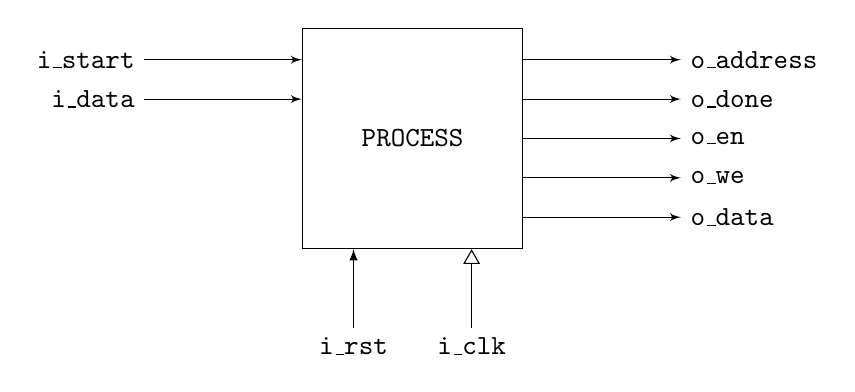
\begin{tikzpicture}[node distance = 5mm and 15mm]
        \node (comp) [draw,minimum size=28mm] {\texttt{PROCESS}};
        % in
        \coordinate[above left= 10mm and 20mm of comp.west]  (i1);
        \foreach \i [count=\xi from 1] in {2} 
            \coordinate[below=of i\xi]  (i\i);
        \foreach \i [count=\xi from 1] in {\texttt{i\_start}, \texttt{i\_data}}
            \draw[-latex']  (i\xi) node[left] {\i} -- (i\xi-| comp.west);
        %under
        \coordinate[below right = 10mm and 7.5mm of comp.south]  (u1);
        \foreach \i [count=\xi from 1] in {2} 
            \coordinate[left=of u\xi]  (u\i);
        %\foreach \i [count=\xi from 1] in {\texttt{i\_clk}, \texttt{i\_rst}}
            \draw[-open triangle 60]  (u1) node[below] {\texttt{i\_clk}} -- (u1 |- comp.south);
            \draw[-latex]  (u2) node[below] {\texttt{i\_rst}} -- (u2 |- comp.south);
            
        % out
        \coordinate[above right= 10mm and 20mm of comp.east]  (o1);
        \foreach \i [count=\xi from 1] in {2,...,5} 
            \coordinate[below=of o\xi]  (o\i);
        \foreach \i [count=\xi from 1] in {\texttt{o\_address}, \texttt{o\_done},
                                                    \texttt{o\_en}, \texttt{o\_we}, \texttt{o\_data}}
            \draw[-latex'] (comp.east |- o\xi) -- (o\xi) node[right] {\i};
        %
        \end{tikzpicture}

    \caption{Schema del componente realizzato.}
    \label{fig:component}
\end{figure}

\end{document}